%%%%%%%%%%%%%%%%%%%%%%%%%%%%%%%%%%%%%%%%%%%%%%%%%%%%%%%%%%%%%%%%%%%%%%%%%%%%%%%%
% experiment.tex: Chapter describing the experiment
%%%%%%%%%%%%%%%%%%%%%%%%%%%%%%%%%%%%%%%%%%%%%%%%%%%%%%%%%%%%%%%%%%%%%%%%%%%%%%%%
\chapter{\gls{ldmx-full}}
\label{chapter:ldmx:experiment}

\gls{ldmx} is a proposed fixed-target experiment aiming to definitively explore
the light dark matter phase space. Even as a proposed experiment, it has a detailed
plan for construction, a beam already in construction, and well established connections
with current technologies used within \gls{hep}. While \gls{ldmx} is not yet built,
it has a well formulated simulation infrastructure that can realistically model
how the detector design responds to various types of interactions happening within it.

\section{The Beam Line}
\todo[inline]{Huge caveat on this section.}
\gls{ldmx} is situated at the end of the Linear Accelerator (Linac) at SLAC National Accelerator
Laboratory. The SLAC Linac can high energy, high rate, and low intensity electron beams for
the various experiments it hosts. Specifically, the Linac Coherent Light Source (LCLS) is
used to guide the beam (of a certain energy) towards the experimental hall - the upgraded
phase of LCLS (LCLS II \cite{lcls-ii}) is currently under construction and is what will
be used for running with \gls{ldmx}.

The experiment is hosted in End Station A (ESA) at SLAC which requires an additional
upgrade to the Linac in order to recieve its beam. LESA (Linac to ESA) \cite{lesa-design}
is also currently being constructed and will be ready for test beam in early 2025.

\section{Detector Design}
LDMX is a missing momentum experiment and its design is focused on measuring
\emph{both} the incoming and outgoing momenta of charged particles interacting
with a thin target.
This design has led to four subsystems each with specialized roles.
\begin{enumerate}
    \item \textbf{Trigger Scintillator} Count the number of electrons incident on the target in time to make a trigger decision.
    \item \textbf{Tracker} Measure charged particle momenta both before (``Tagger'') and after (``Recoil'') the target.
    \item \textbf{Electromagnetic Calorimeter} (\gls{ecal}) Measure the total energy of electrons, positrons, and photons.
    \item \textbf{Hadronic Calorimeter} (\gls{hcal}) Veto additional particles difficult for other subsystems to measured (muons, pions, hadrons,...).
\end{enumerate}
\cref{fig:ldmx-det} displays these subsystems in a diagram along with a representation of
a dark brem interaction occurrring within the target.

The Trigger Scintillator (yellow-orange in \cref{fig:ldmx-det}) is made of layers of vertically segmented bars of plastic
scintillator. Thes layers are arranged in pairs where the layers within each pair are offset from one
another to cover any gaps between the bars. These bars are readout in time to be used within
a trigger decision.\todo{What is a ``trigger'' and how do these bars help?}

The Tracker (purple in \cref{fig:ldmx-det}) is a thin silicon strip detector modeled after
the \gls{hps} tracker. These silicon strips are also arranged in layer pairs where one layer
is angled slightly askew relative to the other in the pair to enable reconstruction of three
dimensional hit locations. The part of the tracker upstream of the target (to the left in \cref{fig:ldmx-det})
is named the ``tagger'' since its purpose is to measure the incident electrons' momenta,
rejecting electrons' with momentum below $30\%$ of the expected beam momentum. The tagger
is situated within the bulk of the magnetic field enabling highly precise measurement of
this incident momentum. The other part of the tracker located downstream of the target
(to the right in \cref{fig:ldmx-det}) is named the ``recoil'' tracker since its job is
to measure the momenta of all charged particles recoiling from interactions within the
target. While it is not located within the magnet volume, it is still situated within
the fringe field, allowing functional momentum resolution.

The \gls{hcal} (green in \cref{fig:ldmx-det}) is a sampling calorimeter made up of alternating layers of steel absorber and
plastic scintillator bars. The \gls{hcal} is further subdivided into the ``side'' \gls{hcal} which
is situated around the \gls{ecal} and the ``back'' \gls{hcal} downstream of the \gls{ecal}. The back \gls{hcal}
has the orientation of the scintillator bars alternate between vertical and horizontal
so that clusters and tracks can have three-dimensional coordinates more preceisely identified.

The \gls{ecal} (blue in \cref{fig:ldmx-det}), as a primary volume of interest within the analysis discussed here, is given its
own section below \cref{sec:ldmx:ecal}.

\begin{figure}
    \centering
    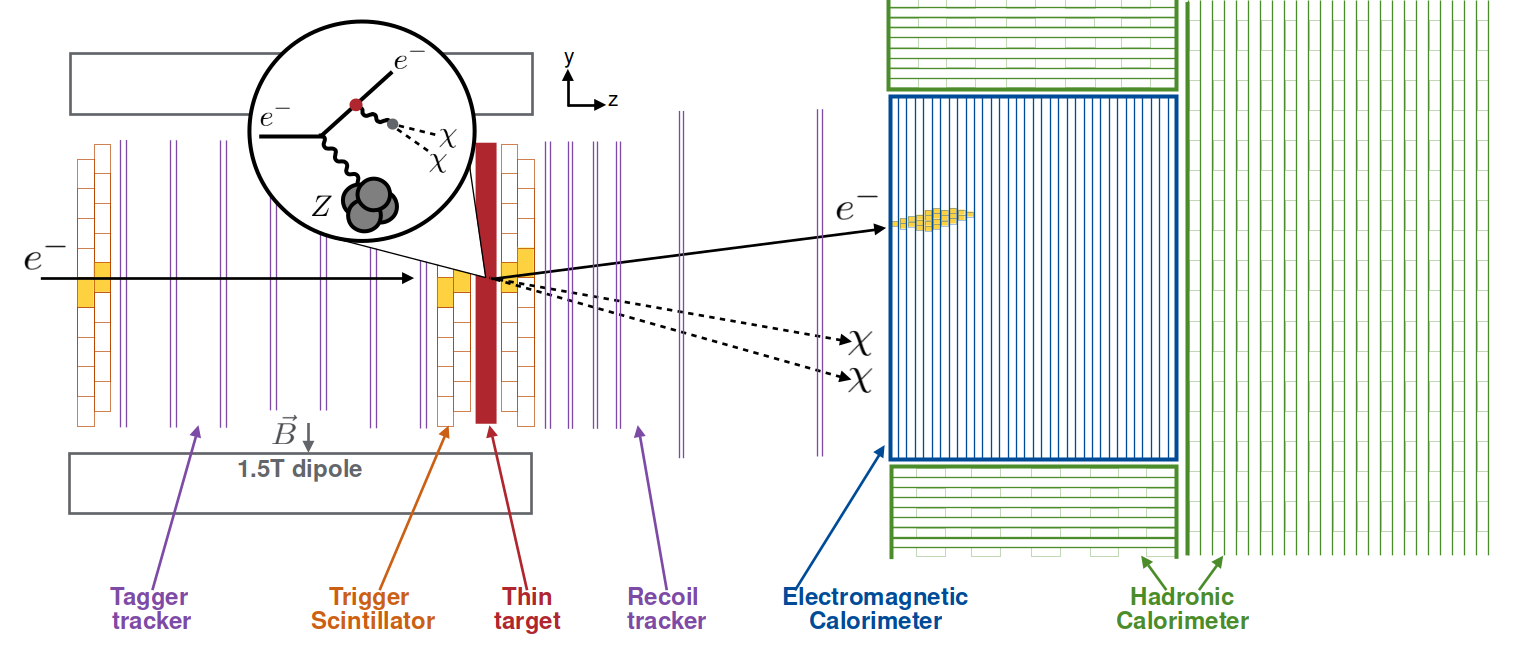
\includegraphics[width=0.9\textwidth]{figures/ldmx/experiment/detector.png}
    \caption{
        Diagram of LDMX detector apparatus with a representation of a signal event where
        a dark brem occurs within the target. Diagram is not to scale. Credit to Christian Herwig
        for original development of diagram.
    }
    \label{fig:ldmx-det}
\end{figure}

\section{\gls{ecal}}
\label{sec:ldmx:ecal}

More detail about \gls{ecal} since it relates to the ME search later.

\begin{figure}
    \centering
    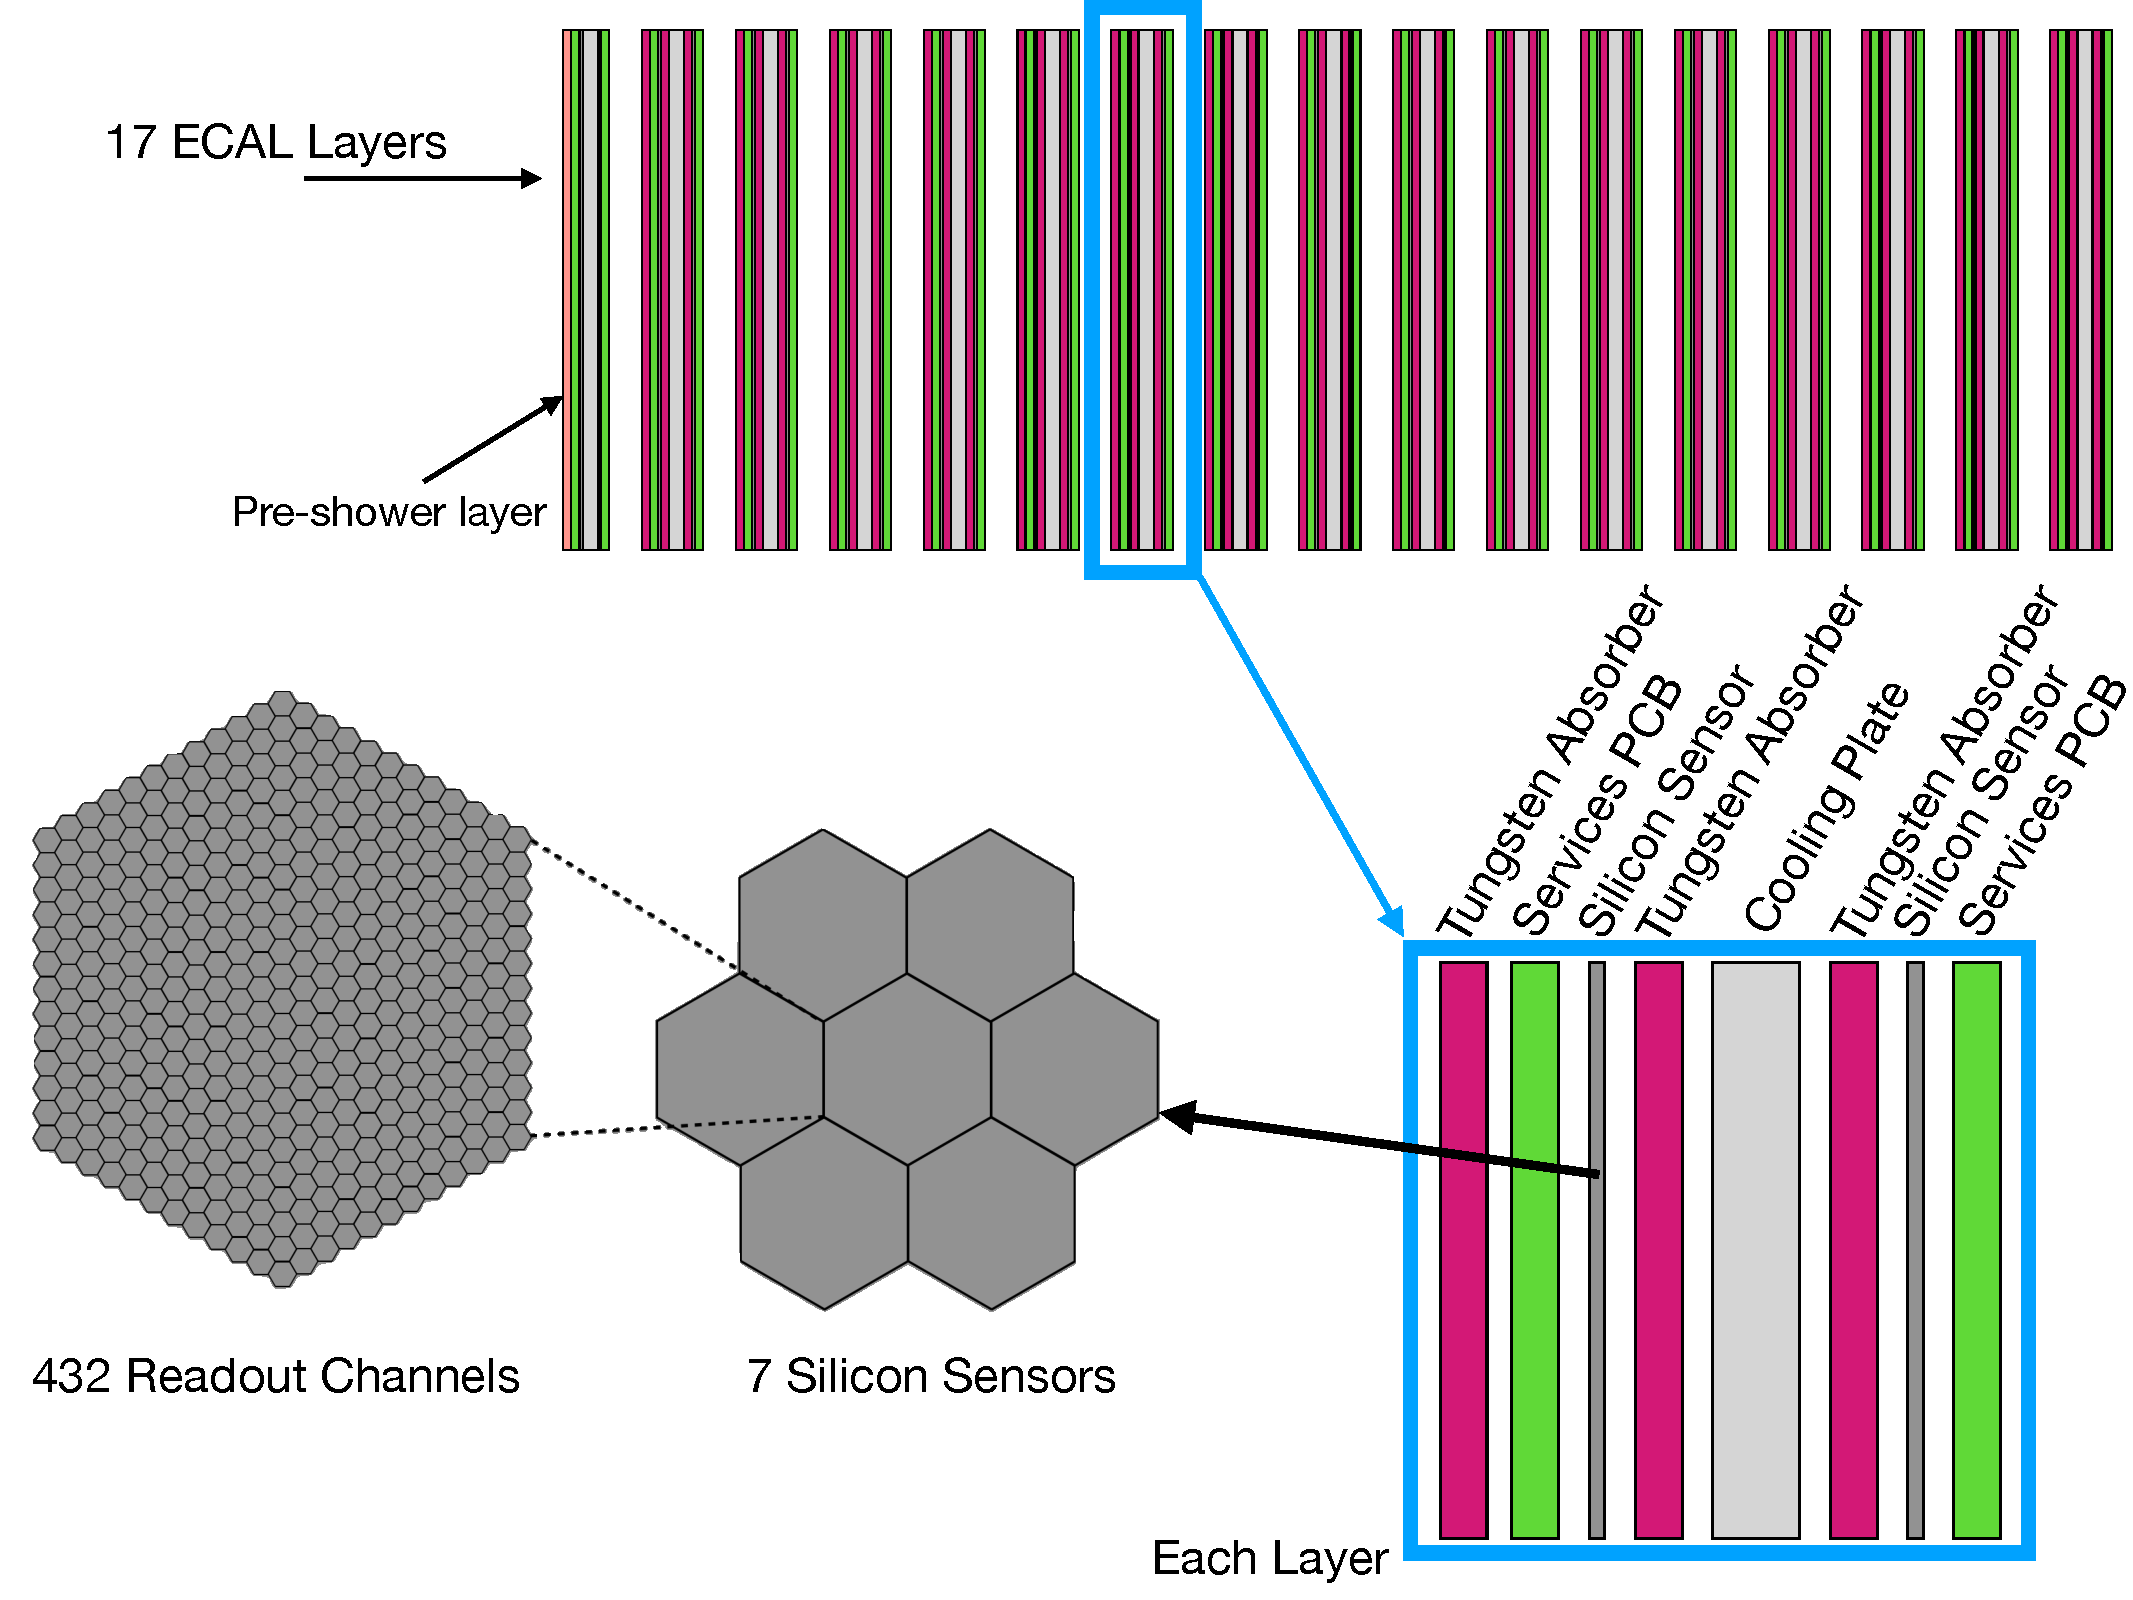
\includegraphics[width=0.9\textwidth]{figures/ldmx/experiment/ecal.pdf}
    \caption{
        Diagram of LDMX \gls{ecal} construction showing the longitudinal segmentation
        (top and bottom right) and the transverse segmentation (bottom left).
        Credit to Joe Muse.
    }
    \label{fig:ldmx-ecal}
\end{figure}
%%%%%%%%%%%%%%%%%%%%%%%%%%%%%%%%%%%%%%%%%%%%%%%%%%%%%%%%%%%%%%%%%%%%%%%%%%%%%%%%
